\chapter{Methodology and development}
\label{cha:chapter3}

\section{The Repository}

This work was done in Jupyter notebook format in a GitHub repository (\url{https://github.com/gperaza/road-network}). This repository's root contains an environment definition file and a notebooks folder. Within that folder, the repository contains one folder for the work done in Mérida, Yucatán, and other folder for the different cities in México that are beyond the scope of this report. The following notebooks are included in the Mérida folder:

\begin{enumerate}
	\item Data preparation, downloading/modeling and calculating network stats of Mérida's road network and its urban AGEBs.
	\item Analysis of the road network of Mérida and its urban AGEBs.
	\item Cluster analysis of the urban AGEBs.
\end{enumerate}

To run the code examples in this resource repository, we simply run everything in a pre-built Anaconda environment. This process is detailed in the following section.

\section{The Environment}

This project's repository contains an Anaconda environment file (i.e., .yml) for running the Jupyter notebooks on any computer. Anaconda \cite{anaconda} is a data science platform that facilitates package management and deployment. It is available for Windows, Linux and macOS. We use the Individual Edition, which is the open-source distribution of Anaconda.

First, download and install Anaconda Individual Edition. Once it is installed and running on your computer, run the following code in the terminal window:

\begin{lstlisting}[language=bash]
$ conda config --add channels conda-forge
$ conda env create --file road-network-project.yml
$ conda activate road-network-project
$ jupyter lab
\end{lstlisting}

Once you are in the active environment, open your computer's web browser and visit \url{http://localhost:8888} to access Jupyter Lab and open this work's notebook files.

\section{Data Collection}

This work uses OSMnx to download the street network of Mérida and its AGEBs, construct a graph model of it (using NetworkX), correct, analyze, and visualize at municipal, and neighborhood (AGEB) scales. 

In order to get the street network of Mérida, we define a function to download and save the graph of the municipality, or, if already present, load it as an NetworkX graph object:

\begin{lstlisting}[language=Python]
def get_roads_osmnx(places, update=False, proj=False, crs=None):

	dirpath = pathlib.Path('./data/networks/')
	filepath = dirpath/'merida-road.graphml'
	logpath = dirpath/'log'

	if filepath.exists() and not update:
		G = ox.load_graphml(filepath)
	else:
		# get drivable public streets network, aka road network, without service roads,
		# e.g. private, parking lots, etc.
		# use retain_all if you want to keep all disconnected subgraphs (e.g. when your places aren't adjacent)
		G = ox.graph_from_place(places, network_type='drive')
		ox.save_graphml(G, filepath=filepath, gephi=False)
	
	if proj:
		G = ox.project_graph(G, to_crs=crs)
	
	print(f"Graph created at: {G.graph['created_date']}")
	return G, *ox.graph_to_gdfs(G)
	
places = [{'county' : 'Merida', 'state' : 'Yucatan', 'country' : 'Mexico'}]
G_proj, nodes_proj, edges_proj = get_roads_osmnx(places, update=False, proj=True, crs=3857)
\end{lstlisting}

OSMnx geocodes the query "Merida, Yucatan, Mexico" to retrieve the place boundaries of that city from the Nominatim API, retrieves the drivable street network data within those boundaries from the Overpass API, constructs a graph model (via NetworkX), then simplifies/corrects its topology such that nodes represent intersections and dead-ends, and edges represent the street segments linking them. It also saves the constructed graph as a GraphML file to not re-download the same data again.

OSMnx models all networks as NetworkX MultiDiGraph objects. You can convert to:

\begin{itemize}
	\item Undirected MultiGraphs.
	\item DiGraphs without (possible) parallel edges.
	\item GeoPandas node/edge GeoDataFrames.
\end{itemize}

In the function, we also convert the graph to node and edge GeoDataFrames. Additionally, we project the graph to the WGS84 Pseudo-Mercator  CRS.

Remember that one of the most commonly used CRS is the WGS84 latitude-longitude projection. This can be referred to using the authority code "EPSG:4326". However, such EPSG is in degree units. For that reason, we will use an alternative option which is the "EPSG:3857" that is measured in meters. This projected coordinate system is the one that Google, OpenStreetMap, Bing, ArcGIS, ESRI, etc. use for rendering their maps \cite{epsg3857}.

In the case of the Mérida's urban AGEBs, we collect geographic data from the Institute of Statistics and Geography's (INEGI) National Geoestatistical Framework (MG) and socio-demographic data from INEGI's 2020 Population and Housing Census (2020 Census) conducted from March 2 to March 27, 2020 \cite{2020census}.

The MG is a mexican unique national system designed by INEGI to correctly reference statistical information from censuses and surveys with the corresponding geographic locations \cite{manualMGN}. It is conformed by geostatistical areas divided into three dissaggregation areas (see Figure \ref{fig:MGN_divisions}):

\begin{itemize}
	\item State geoestatistical areas (AGEE).
	\item Municipal geoestatistical areas (AGEM).
	\item Basic geoestatistical areas (AGEB).
	\begin{itemize}
		\item Rural AGEB.
		\item Urban AGEB.
	\end{itemize}
\end{itemize}

\begin{figure}[h!]
	\centering
	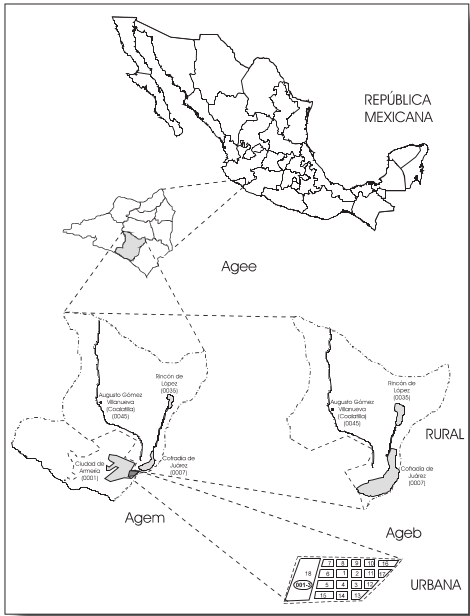
\includegraphics[width=0.6\textwidth]{Figures/MGN_divisions.png}
	\caption{MG dissaggregation areas. Retrieved from: \cite{manualMGN}.
		\label{fig:MGN_divisions}}
\end{figure}

Urban AGEBs are the geographic area, subdivision of municipal areas, occupied by a set of blocks, generally ranging from 1 to 50, perfectly delimited by streets, avenues, walkways or any other easily identifiable feature on the ground and whose land use is mainly residential, industrial, services, commercial, etc., only assigned within urban localities (see Figure \ref{fig:ageb_division}).

\begin{figure}[h!]
	\centering
	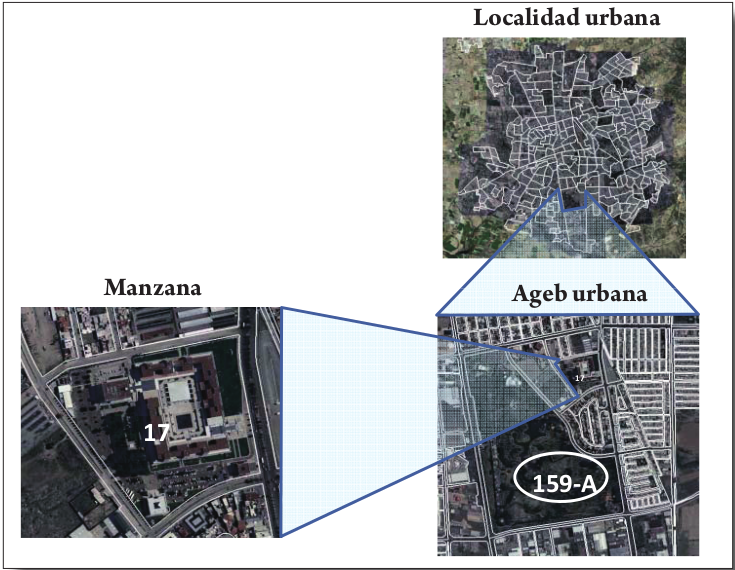
\includegraphics[width=0.7\textwidth]{Figures/ageb_division.png}
	\caption{Urban AGEB dissaggregation areas. Retrieved from: \cite{manualMGN}.
		\label{fig:ageb_division}}
\end{figure}

We download the MG data from \cite{MG_data}, which contains the shapefiles of every dissaggregation area of every mexican state. It is made up of 32 folders, each one named by the geoestatistical key of the federal entity (from 1 to 32), with a national total of 2,469 municipal geoestatistical areas, 45,397 polygons of rural localities, and 4,911 polygons of urban localities, 295,779 points of rural localities, 350 polygons of island territory, 17,469 basic rural geostatistical areas, 63,982 basic urban geostatistical areas and 2,513,853 urban and rural blocks (including scattered hamlets); the information maintains associated names and geostatistical keys as attributes.

The MG references every dissaggregation area with a unique numeric key. The structure of such geostatistical key is represented in Figure \ref{fig:key_structure}.

\begin{figure}[h!]
	\centering
	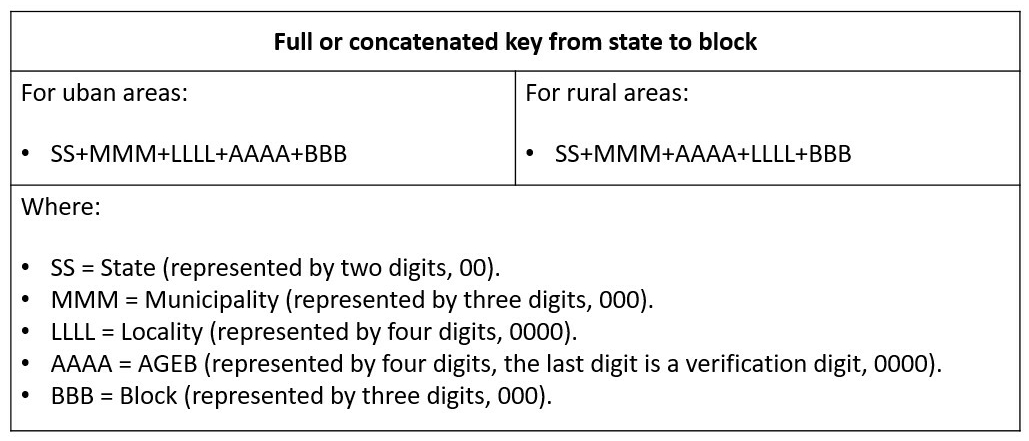
\includegraphics[width=0.8\textwidth]{Figures/key_structure.jpg}
	\caption{MG's geostatistical key structure. Retrieved from: \cite{manualMGN}.
		\label{fig:key_structure}}
\end{figure}


Every state folder of the MG is composed of three subfolders:

\begin{itemize}
	\item Catalogs (catálogos): contains the product catalogs and documentation.
	\item Data set (conjunto\_de\_datos): contains 32 folders, each one corresponding to the state geoestatistical key.
	\item Metadata (metadatos): contains 32 files, each one with the corresponding state geostatistical key, in xml and txt format, and a generic metadata with national information.
\end{itemize}

The file names are formed with the state geoestatistical key and the following suffixes of the file content: 

Where \textbf{ee} corresponds to the state geoestatistical key (from 01 to 32).

\begin{table*}[h!]
	\centering
	\label{tab:MG_filenames}
	\footnotesize
	\begin{tabular}{ l l }
		ee\textbf{ent} & State geoestatistical areas \\
		ee\textbf{mun} & Municipal geoestatistical areas \\
		ee\textbf{ar} & Basic rural geoestatistical areas \\
		ee\textbf{l} & Polygon of urban and rural localities \\
		ee\textbf{lpr} & Rural point locations \\
		ee\textbf{ti} & Island territory\\
		ee\textbf{a} & Basic urban geoestatistical areas \\
		ee\textbf{m} & Block polygons\\
		ee\textbf{fm} & Block fronts \\
		ee\textbf{e} & Road axes \\
		ee\textbf{cd} & Scattered hamlet \\
		ee\textbf{sia} & Complementary area-type services and information (green areas, medians, traffic circles) \\
		ee\textbf{sil} & Complementary line-type services and information
		(rivers, railroads, streams) \\
		ee\textbf{sip} & Complementary point-type services and information
		(municipal palaces, parks or gardens, etc.) \\
		ee\textbf{pe} & External polygon \\
		ee\textbf{pem} & External polygon of blocks \\
	\end{tabular}
\end{table*}

Layers with suffix \textbf{ti}, \textbf{cd}, \textbf{pe}, \textbf{pem}, \textbf{sia}, \textbf{sil}, \textbf{sip}, are included only if the locality has this type of information.

INEGI's 2020 census data was downloaded from \cite{2020census} on the main results by AGEB and urban block subsection. In this subsection we can download data from every mexican state in a CSV (comma-separated values) file.

In this work, we are only using the MG Yucatán folder (31\_yucatan) and the file of the basic urban geoestatistical areas (31a.shp), as well as census data from Yucatán.


\section{Data Exploration and Preparation}

Mérida's street network has 93485 edges and 35105 nodes, and covers a convex hull area of 1,032.4 km$^2$ that comprises the 874.4 km$^2$ of the Mérida municipality's area \cite{2020census}. However, the network is disconnected due to unfinished roads or roads at the boundary. Thus, we retain only the largest connected component, which has 93371 edges and 35031 nodes, comprising the 99.9\% of edges and 99.8\% of nodes from the whole network. The covered area is the same. 

In order to perform some analysis involving how street network metrics change with scale, we import AGEBs from the MG to create a subgraph for each different AGEB. Additionally, we want to include socio-demographic data to the analysis. However, the census dataset does not include the polygons of the AGEBs. For such reason, we must merge both MG and 2020 Census data.

When we import the 2020 Census data, we encounter missing information recorded as * (asterisk) or N/D (Not Available). What we did, was to replace such values with a zero (0). After that, we changed the data types of the information, which can be consulted in \cite{census_data}, from string to float for further analysis. We also filter the data by dropping the totals by municipality and locality as we only need totals by AGEB.

In order to merge the data from the 2020 Census and the MG, we create a new column in the 2020 Census dataframe where we took values from the geostatistical keys of state, municipality, locality, and AGEB to conform the concatenated (full) geostatistical key. In this case, we do not take into account the blocks. We add missing zeros to the values of the municipality and locality geostatistical key to fulfill the appropiate length. Also, we change the data types of the state, municipality, and locality geostatistical keys from integer to string to concatenate them. Next, we drop columns from the 2020 Census dataframe that will be duplicated after the merging. Finally, we perform the merge with the MG dataframe on the concatenated geostatistical key column present in both dataframes using the inner merge type that uses the intersection of columns from both dataframes, similar to a SQL inner join \cite{pandas_merge}.

The MG has geometric data from 1532 AGEBs, while the 2020 Census has data from 1432 AGEBs. After the merge, we ended up with 1432 AGEBs. Important to notice that these AGEBs are from all the Yucatán state. But, as this work is focused on Mérida, we select only its AGEBs. After filtering for Mérida's AGEBs, we ended up with 523 urban AGEBs. This merged geodataframe was saved as shapefiles under the name \textit{merida\_ageb\_census\_data.shp} with the Pseudo-Mercator projection.

To get the subgraphs for each AGEB, we add a column containing the calculated area, in meters, of the AGEB based on its polygon. Next, we project the geodataframe to the Mercator projection, which is in degree units, because our data must be in such projection to download the network with OSMnx. Then, we create queries from the AGEBs geodataframe to automate the downloading and saving of AGEB's road networks. The queries contain the path where graphs will be saved, the polygon of the AGEB to be downloaded, and the area in meters of the AGEB. Every graph will be saved as shapefiles and GraphML format. After getting the AGEB graphs, we ended up having 517 AGEBs because some AGEBs did not have nodes and, or edges within the requested polygon. The making and saving of AGEB graphs lasted around 32 minutes.

OSMnx includes two modules (basic and extended stats) for calculating geometric and topological network measures for street network analysis. The list of the measures is the following:

\begin{itemize}
	\item Number of nodes.
	\item Number of edges.
	\item Average node degree.
	\item Number of intersections: nodes with $>$1 physical streets connected to them.
	\item Average streets per node: how many physical streets (edges in the undirected representation of the graph) connect to each node (i.e., intersection or dead-end) on average.
	\item Streets per node count: number of physical streets connecting to a node.
	\item Streets per node proportion: same as previous but proportion of the total, rather than counts.
	\item Total edge length: sum of all edge lengths in graph, in meters.
	\item Average edge length: mean edge length in the graph, in meters.
	\item Total street length: sum of all edges in the undirected representation of the graph.
	\item Average street length: mean edge length in the undirected representation of the graph, in meters.
	\item Street segments count: number of edges in the undirected representation of the graph.
	\item Node density: number of nodes divided by area in km$^2$.
	\item Intersection density: intersection count divided by area in km$^2$.
	\item Edge density: Total edge length divided by area in km$^2$.
	\item Street density: Total street length divided by area in km$^2$.
	\item Average circuity: Total edge length divided by the sum of the great circle distances between the nodes of each edge.
	\item Self-loop proportion: proportion of edges that have a single node as its endpoints (i.e., the edge links nodes u and v, and u==v).
	\item Clean intersection count: number of intersections in street network, merging complex ones into single points.
	\item Clean intersection density: clean intersection count divided by area in km$^2$.
	\item Average neighbor degree.
	\item Average neighbor degree average.
	\item Average weighted neighbor degree.
	\item Average weighted neighbor degree average.
	\item Degree centrality.
	\item Average degree centrality.
	\item Clustering coefficient.
	\item Average clustering coefficient.
	\item Weighted clustering coefficient.
	\item Average weighted clustering coefficient.
	\item PageRank.
	\item Maximum PageRank node.
	\item Maximum Pagerank.
	\item Minimum PageRank node.
	\item Minimum PageRank.
	\item Node connectivity.
	\item Average node connectivity.
	\item Edge connectivity.
	\item Eccentricity.
	\item Diameter.
	\item Radius.
	\item Center.
	\item Periphery.
	\item Closeness centrality.
	\item Average closeness centrality.
	\item Betweenness centrality.
	\item Average betweenness centrality.
\end{itemize}

We calculate the listed metrics for the Mérida municipality street network, except for node and edge connectivity, eccentricity, diameter, radius, center, and periphery due to exhaustion of the computer memory. The calculations lasted around 6 hours and 7 minutes. We saved the calculations in a csv file to not recalculate them again.

For the calculation of metric for AGEBs, we do not exclude any listed metric. Such calculations lasted around 47 minutes for all AGEBs. However, two AGEBs were excluded because they had only one node. Also, when we updated the local degree, betweenness and closeness centrality to global, other two AGEBs were excluded as Mérida's street network did not include any node of such AGEBs. For such reason, we ended up working with 513 AGEBs in this work. Finally, we merge the network calculation with the 2020 Census and MG data into a single geodataframe, and a column for population density was added. The data was saved in shapefiles named \textit{merida\_ageb\_stats\_census.shp}.

\section{Data Modeling}

As one of our objectives is to perform a clustering algorithm on the AGEBs to find similar AGEBs based on socio-demographic data and their network measures, we must choose how our AGEBs are going to be interconnected.

Spatial weights are used to represent geographical relationships between two spatial observations. We consider two different approaches to construct spatial weights based on contiguity/adjacency relations. Such approaches arises from the legal moves that different chess pieces can make. Rook contiguity considers two polygons as connected if they share an edge on their border (see Figure \ref{fig:rook-contiguity}). But Queen contiguity connects two polygons if they share a one or more points on their border (see Figure \ref{fig:queen-contiguity}). As result, queen representation has more neighbors than rook has. We chose a rook representation as it exploits the sparse nature of contiguity weights matrices \cite{rey_geo_ds_2020}.

\begin{figure}[h!]
	\centering
	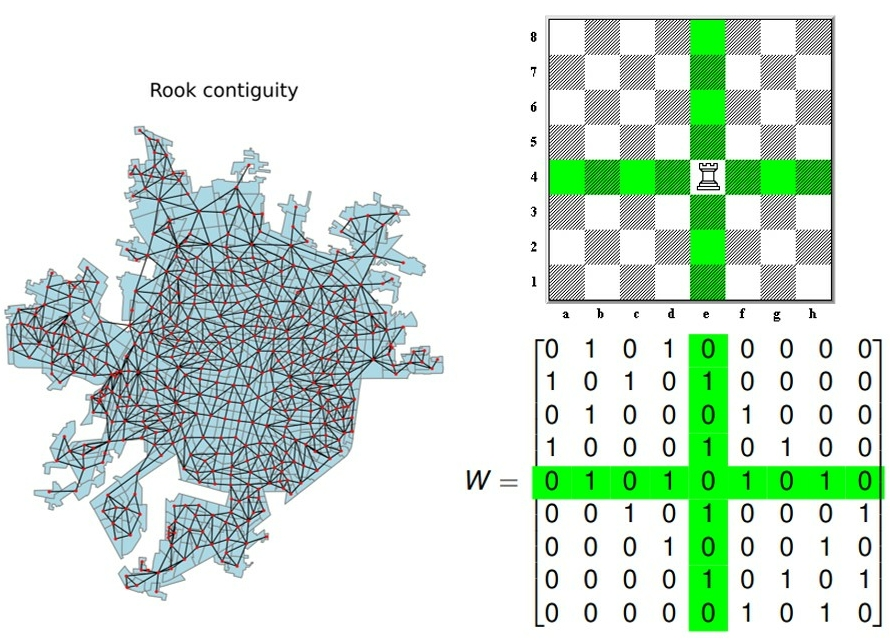
\includegraphics[width=0.8\textwidth]{Figures/rook-contiguity.jpg}
	\caption{Rook contiguity.
		\label{fig:rook-contiguity}}
\end{figure}

\begin{figure}[h!]
	\centering
	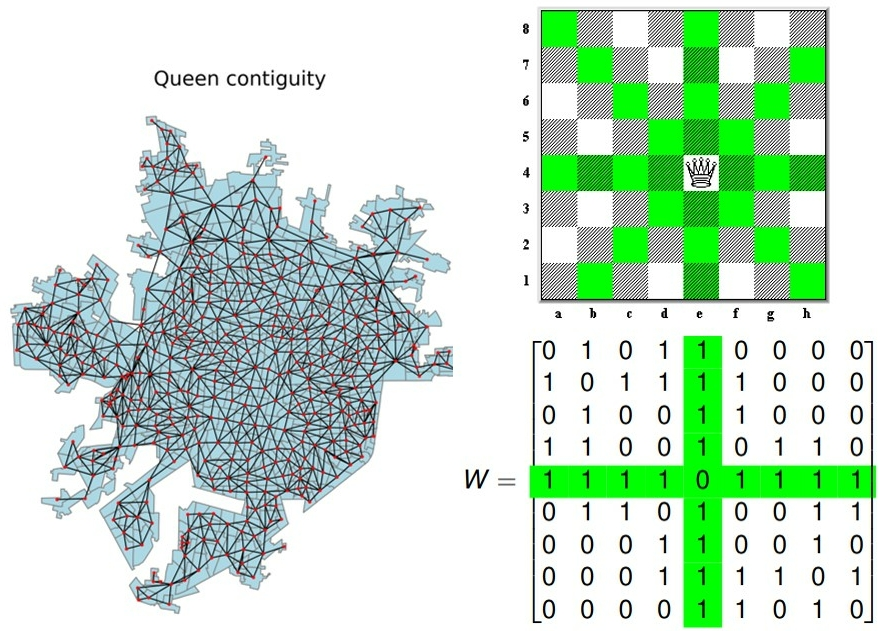
\includegraphics[width=0.8\textwidth]{Figures/queen-contiguity.jpg}
	\caption{Queen contiguity.
		\label{fig:queen-contiguity}}
\end{figure}

When we construct the rook adjacency matrix, we had to eliminate some AGEBs that were disconnected (islands). We drop AGEBs from Mérida localities such as San José Tzal, Komchen, Chablekal, as well as the Military Base and the Airport of Mérida. The adjacency matrix is used to add connectivity constraints to the clustering algorithm to impose a certain structure defining for each sample the neighboring samples. Also, it makes the algorithm faster.

The clustering algorithm that we use in this work is the hierarchical clustering (also known as connectivity-based clustering) that builds nested clusters by merging or splitting them recursively. The hierarchy of clusters is represented as a tree (or dendrogram). A machine learning Python library, called Scikit-Learn \cite{scikit-learn}, provides us their implementation of the agglomerative hierarchical clustering algorithm. 

The agglomerative clustering is the most common type of hierarchical clustering used to group objects in clusters based on their similarity. It uses a bottom-up approach: each observation starts in its own cluster, then pairs of clusters are successively merged until all clusters have been merged together \cite{hierarchical_scikit}. The linkage criteria determines the metric used for the merge strategy:

\begin{itemize}
	\item \textbf{Ward} minimizes the variance of the clusters being merged.
	\item \textbf{Maximum} or \textbf{complete linkage} minimizes the maximum distance between observations of pairs of clusters.
	\item \textbf{Average linkage} minimizes the average of the distances between all observations of pairs of clusters.
	\item \textbf{Single linkage} minimizes the distance between the closest observations of pairs of clusters.
\end{itemize}

We select ward linkage as the most suitable because we only have an adjacency matrix, not a distance matrix.

The final step was to find the appropiate number of clusters for the algorithm. Based on empirical observation, 14 clusters were selected as they best describe similarity between AGEBs.

